\section{Incremental Workflow Mining with Petri Nets}
Another relevant to my research approach is implemented by Rubin et al. \cite{citeulike:1885717} and called \textit{incremental workflow mining}. Authors built their system using a business process mining framework ProM by van Dongen et al. \cite{citeulike:5043673} which synthesizes a Petri Net corresponding to the process observed from a transition system discovered through the Software Configuration Management (SCM) system mining. While the SCM system mining is rather high-level engineering process mining due to the granularity of artifacts kept in the system, the approach discussed is very promising for the modeling software processes from the low-level product and process data.

\begin{figure}[tbp]
   \centering
   \includegraphics[height=65mm]{petri.eps}
   \caption{Illustration of the ``Generation and Synthesis Approach'' from \cite{citeulike:5043673}: a) Transition System with regions shown; b),c) Petri Nets.}
   \label{fig:petri}
\end{figure}

On the first step of the designed algorithm, Rubin et al. map the audit trail information from the SCM system into the event chain which corresponds to the software process artifacts. Authors call this process as \textit{abstraction on the log level} which is implemented as a set of filters which not only aggregate basic events into the high-level entities but also remove irrelevant information (noise). 

The event chain constructed through the abstraction then treated with the ``Generate and Synthesis'' \cite{citeulike:3718014} approach. The algorithms used for the transition system synthesis are also based on the history (prefix) and the future (suffix) sequences of events related to the current one. Applied to the abstracted log information these algorithms are generating a rather large graphs (transition systems) where edges are connecting observed events. These transition systems then succesively simplified by using varios reduction strategies: ``Kill Loops'', ``Extend'', ``Merge by Output'', and their combinations.

At the last step of the algorithm Transition Systems are converted into the Labeled Petri Nets where different transition can refer to the same event.




An
important quality of the first step is that, unlike existing approaches, it can be
tuned towards the application. Depending on the desired qualities of the model,
the algorithm can be tuned to provide suitable models.